% Author:: Sebastien Badia (<seb@sebian.fr>)
% Date:: 2014-04-02 01:36:20 +0200
% vi: set ft=tex :

\section{Openstack}
\begin{frame}{Outline}
    \tableofcontents[currentsection,hideallsubsections]
\end{frame}
\subsection{Introduction}

\begin{frame}{OpenStack}
  \begin{textblock}{}(11,5)
      
\includegraphics[width=8em]{img/openstack-logo512}
  \end{textblock}
  \begin{itemize}
    \item Infrastructure as a service (\textbf{IaaS}) cloud middleware
      \medskip
    \item Open Source software (\textsl{\textbf{Apache} License})
      \medskip
    \item Derived from \textbf{Nebula} (\textsl{NASA}) and \textbf{Cloud Files} (\textsl{Rackspace})
      \medskip
    \item Written in \textbf{Python}
      \medskip
    \item Stable release: \textsl{\textbf{Havana} (October 13, 2014)}
      \medskip
  \end{itemize}
\end{frame}

\subsection{The foundation}
\begin{frame}{OpenStack Foundation}
  \begin{itemize}
    \item More than \textbf{9500 individual members}
      \medskip
    \item \textbf{100 countries}
      \medskip
    \item \textbf{850 different organizations}
      \medskip
    \item Secured more than \textbf{\$10 million} in funding
      \medskip
    \item Managed by 3 committee
  \end{itemize}
\end{frame}

\subsection{Committee}
\begin{frame}{Technical Committee}
  \begin{textblock}{}(11.5,-1)
      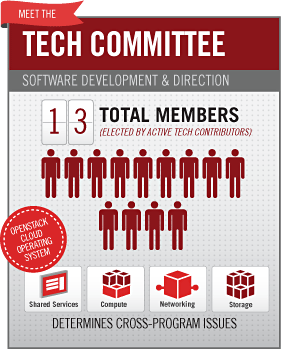
\includegraphics[width=7em]{img/osgraphictech}
  \end{textblock}
  \begin{itemize}
    \item TC manage software development and direction
      \medskip
    \item 13 members elected by active contributors
      \medskip
    \item Each OpenStack project has a PTL\footnote{Project Technical Leader}
      \medskip
    \item 5 are directly elected, and 8 are PTL
      \medskip
    \item Enforce OpenStack ideals (Openness, Transparency, Commonality, Integration, Quality)
  \end{itemize}
\end{frame}

\begin{frame}{Board of Directors}
  \begin{textblock}{}(11,6)
      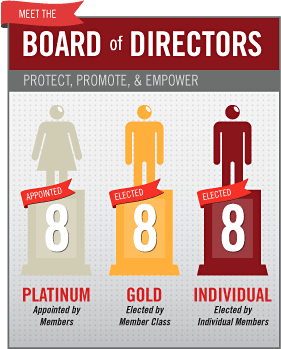
\includegraphics[width=7em]{img/osgraphicboard}
  \end{textblock}
  \begin{itemize}
    \item Protect, promote and empower OpenStack
      \medskip
    \item 24 members to provides strategic and financial oversight of Foundation
      \begin{itemize}
        \item 8 platinum (appointed by members)
        \item 8 gold (elected by member class) (eNovance \Smiley)
        \item 8 individual (elected by individual members)
      \end{itemize}
      \medskip
    \item Leaded by Alan Clark (Suse)
  \end{itemize}
\end{frame}

\begin{frame}{User Committee}
  \begin{textblock}{}(11,3.5)
      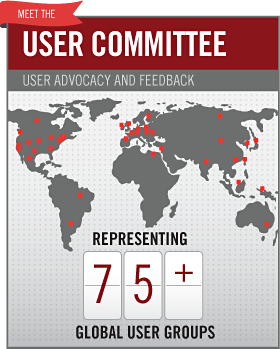
\includegraphics[width=7em]{img/osgraphicusercommittee}
  \end{textblock}
  \begin{itemize}
    \item User advocacy and feedback, anybody can join
      \medskip
    \item Represent a broad set of enterprise, academic and service provider users
      \medskip
    \item Leaded by Tim Bell (CERN)
  \end{itemize}
\end{frame}

\begin{frame}{Community}
  \begin{textblock}{}(8,2)
      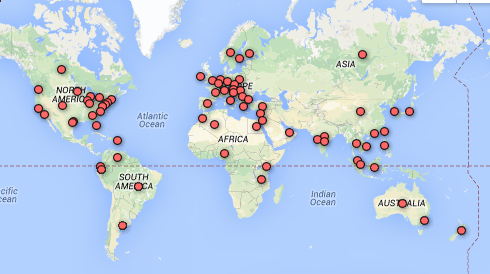
\includegraphics[width=12em]{img/oscommunity}
  \end{textblock}
  \begin{itemize}
    \item \textbf{Core} developers (elected) Grant for merging into master
      \medskip
    \item Anyone can contribute
      \begin{itemize}
        \item Code
        \item Documentation
        \item Support (irc, mail)
        \item …
      \end{itemize}
      \medskip
    \item \url{https://www.openstack.org/community/}
  \end{itemize}
\end{frame}

\begin{frame}{Releases cycle}
  \begin{center}
    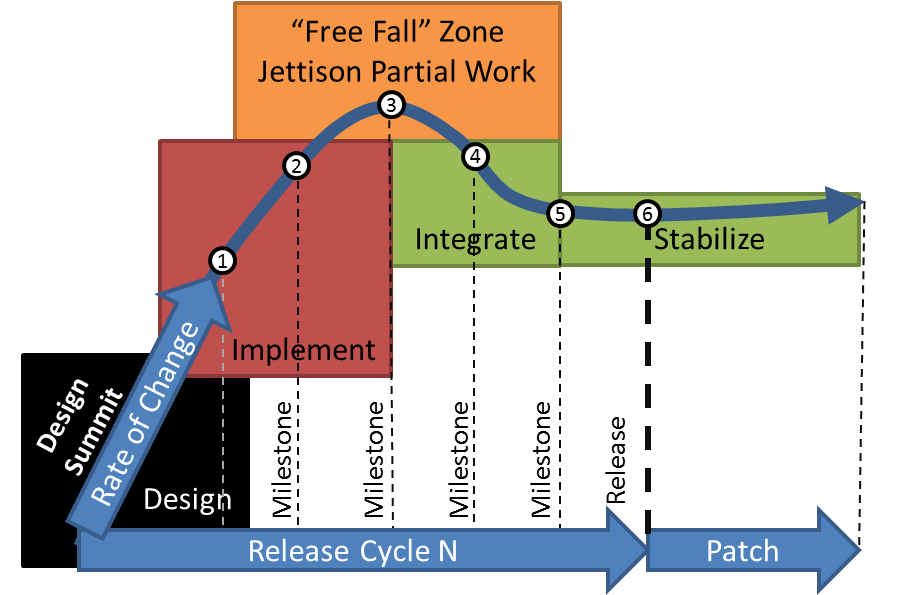
\includegraphics[width=20em]{img/os-releases}
  \end{center}
  \begin{itemize}
    \item A release every 6 months
    \item Alphabetical order \Smiley
    \item \url{https://wiki.openstack.org/Releases}
  \end{itemize}
\end{frame}
